\section{ニコ書を支える本とさや}

人類に最も必要な食料は焼肉です。
チームの絆を深めるために、メンバーが同じ網の肉を食うことはとても重要です。
チームのホーム焼肉屋を設定し、いつでも行けるようにしましょう。

\subsection{本とさや}

本とさやは浅草にある焼肉屋で、それなりに高いけどめちゃめちゃ美味い肉が食えます。
単品では高いんですが、美味いので少量で十分満足できます。
平均予算は5000円くらいですかね。

店に到着するとまず 一品料理の \emph{イカフェ} と、一番高い肉コースの
\emph{A盛り} を頼みます。
イカフェはイカ刺しときゅうりと大根をコチジャンで和えたもので、
ピリ辛で歯ごたえがよく、出てくるのも早いのでお通し代わりに最適です。

A盛りは、タン、ロース、カルビ、骨付きカルビ、ミノのセットで、4〜5人前で11,500円です。
肉はどれも分厚く、しかし口に入れると蕩けるように噛み切れてしまいます。

\begin{figure}[H]
\centering
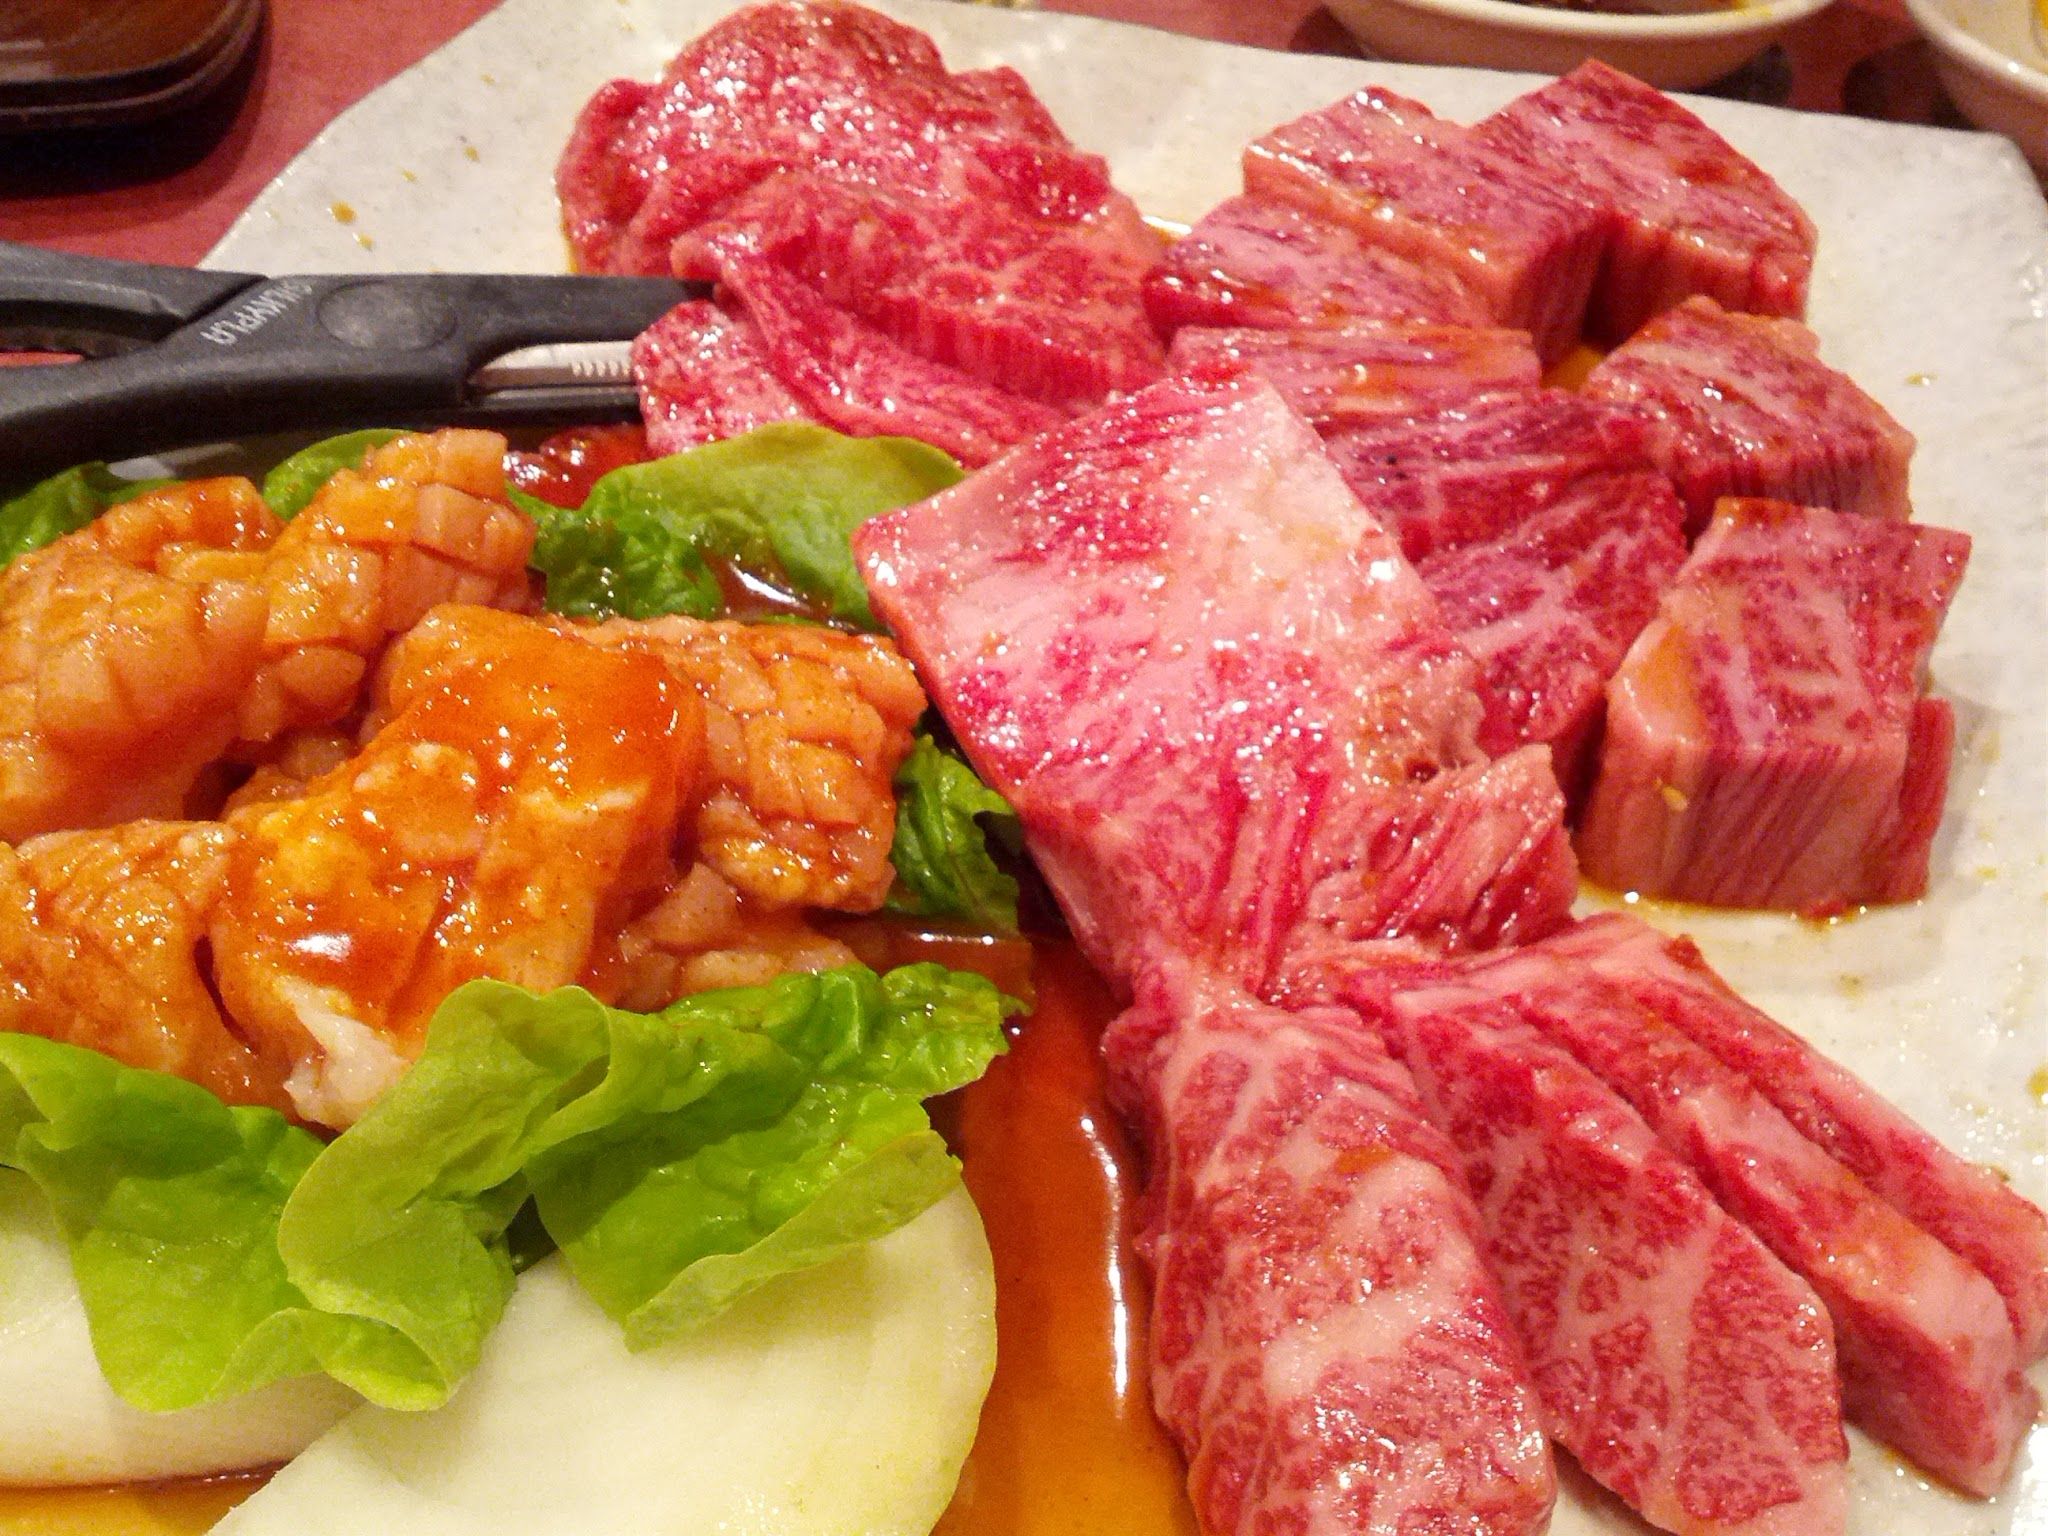
\includegraphics[width=\textwidth]{../images/hontosaya.jpg}
\caption{肉ッ 食わずにはいられないッ}
\end{figure}

A盛りを食いきってもまだ食い足りない場合は、単品の肉を追加します。
上ナントカも美味いのですが、ここで特筆すべきはサービスカルビです。
1人前980円という安さながら、味も良く食べごたえもあるカルビが通常の2人前くらいの量が出てきます。
チェーン店の特上カルビよりもよっぽど美味いですよ。

満腹まで食って料金は5000〜6000円くらいと、
牛角などで「質を量で補う」食い方をした時と料金的にはあまり大差なく、
だいぶお得感は高いと思います。

\subsection{ニコ書の錬金術師}

ニコ書チームには数人の錬金術師がいました。

錬金術とは、飲食代をカードで支払い現金を徴収することで、
来月の自分と現金を(ほぼ)等価交換することです。 錬金術を成功させるには、
それなりに高い金額 (3人でファミレスに行って5000円とかだと
\emph{あとから分割できない} のでリスクが高い) で、
さらに細かい調整がしやすい食事が向いています。
錬金術に最適な料理の1つが焼肉です。

錬金術師とは、つまりお金の管理能力が欠如している人で、
給料日前やカード引き落とし前日にはいつもカネが不足しています。
ニコ書チームでは、複数人の錬金需要が被らないように、
お互いの財務状況を十分考慮しながら、自らの錬金術を高めていきました。

\subsection{肉の名言}

\emph{肉は便利 野菜は草}

徹夜明けの栄養補給には肉を食うのが一番だという教え。
そして野菜は草だから食うなという教え。
